%%  File: main.tex
%%  Author: Matthew Gidden
%%  Created: Sept. 17, 2013
%%  Purpose: Prelim Presenation
     
\documentclass[9pt]{beamer}
\usetheme[white]{Wisconsin}
%\title[short title]{long title}
\title[Cyclus]{An Agent-Based Modeling Framework and Application for the Generic
  Nuclear Fuel Cycle}
%\author[short name]{long name}
\author[MJG]{Matthew Gidden}
%\date[short date]{long date}
\date[09.23.2013]{September 23, 2013}
%\institution[short name]{long name}
\institute[UW-Madison]{University of Wisconsin-Madison}
% Page numbers.
\setbeamertemplate{footline}[page number]
% Those icons  in the references are terrible looking.
\setbeamertemplate{bibliography item}[text]

%% % this is a great way to compile only one (or more) frames at a time as you're
%% % working, saving tons on compile time
%% \includeonlyframes{current}

\begin{document}
%%%%%%%%%%%%%%%%%%%%%%%%%%%%%%%%%%%%%%%%%%%%%%%%%%%%%%%%%%%%%
%% From uw-beamer Here's a handy bit of code to place at 
%% the beginning of your presentation (after \begin{document}):
\newcommand*{\alphabet}{ABCDEFGHIJKLMNOPQRSTUVWXYZabcdefghijklmnopqrstuvwxyz}
\newlength{\highlightheight}
\newlength{\highlightdepth}
\newlength{\highlightmargin}
\setlength{\highlightmargin}{2pt}
\settoheight{\highlightheight}{\alphabet}
\settodepth{\highlightdepth}{\alphabet}
\addtolength{\highlightheight}{\highlightmargin}
\addtolength{\highlightdepth}{\highlightmargin}
\addtolength{\highlightheight}{\highlightdepth}
\newcommand*{\Highlight}{\rlap{\textcolor{HighlightBackground}{\rule[-\highlightdepth]{\linewidth}{\highlightheight}}}}
%%%%%%%%%%%%%%%%%%%%%%%%%%%%%%%%%%%%%%%%%%%%%%%%%%%%%%%%%%%%%

%||||---------------
\frame{
\titlepage
}
%---------------||||

%---------------||||
\section{Introduction}
This chapter seeks to lay out a plan by which a fully agent-based simulation can
be implemented for a generic nuclear fuel cycle with a more realistic chemical
separations and fuel-matching model than currently exists in the field. The term
generic implies that the facilities involved are not known \textit{a priori}
and, accordingly, facilities can be coupled together automatically, separating
the concern of fuel facility modeling and connection from the simulation
solution engine. For example, a modeler has the choice to model a separations
facility and advanced fuel fabrication facility as separate entities whose
connected supply and demand are met by a generic engine, or to model the two
facilities as a single combined and coupled entity. Additionally, the solution
framework for this matching engine must be agnostic as to the classes of
commodities and materials involved. Rather than hard-coding in constraints and
capacities for different material classes, they are added dynamically based on
the entities involved in the simulation-based solution.

As fuel cycle simulators have progressed from simple spreadsheet applications,
work advancing the field has focused on including in-simulation dynamic
calculations of important metrics and parameters in order to provide feedback to
the simulation rather than solely post-processing simulation output. A number of
examples exist. COSI uses the CESAR depletion code \cite{vidal_cesar:_2006} to
automate output fuel characteristics in order to reduce voluminous user input
for simulated materials. Scopatz introduced the notion of essential physics
modeling with his Bright simulation engine \cite{scopatz_essential_2011}. Most
recently, Huff has added to this area of work by developing a repository
facility for the \Cyclus simulator that analyzes repository effects due to
different combinations of materials in different repository
geologies~\cite{huff_integrated_2013}.

This work proposes additional advancement of the dynamic simulation of nuclear
fuel cycles using the \Cyclus simulator. First, a simulation framework for
simulation entity interaction is introduced, the primary goal of which is to
encapsulate simulation-level design decisions. The framework allows for market
interactions to be defined, providing a formalism by which information related
to supply and demand of commodities and materials can be represented in a
general sense. Commodities are not treated simply as quantities, instead the
quantity and \textit{quality} of commodities is treated.  Next, a mathematical
programming formulation based on the multi-commodity transport problem is
proposed to solve the generic supply-demand matching problem. A linear program
formulation and mixed integer-linear program formulation is proposed, the latter
of which addresses the trade-off between computation speed and realism. Finally,
the issue of matching separated elemental streams with requested recycled fuel
is addressed via an approximation linear program.

\section{Fuel Cycle Simulation}
% simulation.tex

\begin{frame}[ctb!]
  \frametitle{Simulating the Nuclear Fuel Cycle} 

  Fuel cycle simulators are designed to answer policy-related questions
  regarding transitions from one equilibrium state to another.

  \vspace{0.2cm}

  \pause
  A simulator answers the following questions as a function of its 
  parameter space:
  \begin{itemize}
    \item how much material exists
    \item where does that material reside
    \item from/to where and when is material transported
    \item what kinds of facilities are needed
    \item when is each type of facility needed
  \end{itemize}
\end{frame}

\begin{frame}[ctb!]
  \frametitle{Simulating the Nuclear Fuel Cycle}
  The nuclear fuel cycle is simulated via \textit{scenarios}.\vspace{0.2cm}

  A scenario generally defines a demand for nuclear power and the types of
  reactors that can respond to that demand. Supporting facilities can be
  explicitly or implicitly modeled to provide fuel for the reactors, and such
  behavior depends on the model used by the simulator.\vspace{0.2cm}

  Some nuclear fuel cycle simulators (FCS) currently in use today:
  \begin{itemize}
    \item CAFCA (MIT) \cite{busquim_e_silva_system_2008}
    \item COSI (CEA) \cite{boucher_cosi:_2006}
    \item DANESS (ANL) \cite{durpel_daness_2003}
    \item VISION (INL) \cite{yacout_vision_2006}
  \end{itemize}
\end{frame}

\begin{frame}[ctb!]
  \frametitle{FCS Metrics}

  FCSs generally report back metrics about the fuel cycle in question. Many of
  these metrics are functions of facility deployment, material flow, and
  material residency, including:

  \begin{itemize}
    \item economics
    \item waste management
    \item sustainability
    \item nonproliferation
  \end{itemize}
\end{frame}

\begin{frame}[ctb!]
  \frametitle{FCS Design Choices}
  Simulation designers are faced with a number of decisions, including:
  \begin{itemize}
    \item facility deployment
    \item fidelity of physical, chemical, and industrial processes
    \item material transaction modeling
  \end{itemize}
\end{frame}

\begin{frame}[ctb!]
  \frametitle{FCS Design Choices: Deployment}

  Reactor deployment choices in almost all cases are chosen by the user.\vspace{0.2cm}

  Supporting facility deployment can be chosen by the user, but in most present
  cases, they are deployed when needed by a look-ahead function.\vspace{0.2cm}

  In many present cases, deployment, although user defined, is restricted by
  future available material. For example, if an advanced reactor requires
  transuranic (TRU) fuel, and a simulation knows that TRU will not be available,
  simulators instead deploy a non-constrained reactor.\vspace{0.2cm}

  In such cases, a class of reactors, e.g. LWRs, is considered never to be
  fuel constrained.
\end{frame}

\begin{frame}[ctb!]
  \frametitle{FCS Design Choices: Fidelity}

  Physical, chemical, and process fidelity are all design choices for simulators.\vspace{0.2cm}

  Physical fidelity includes the choice to model isotopic decay and whether or
  not to model in-core reactor physics.\vspace{0.2cm}

  Chemical and process fidelity include the modeling of the chemical separations
  and advanced fuel fabrication processes. The separations-fuel fabrication
  interface is generally not treated by the current simulator cadre.
\end{frame}

\begin{frame}[ctb!]
  \frametitle{FCS Design Choices: Material Transactions}

  Determining how material flows, or is transacted, is a critical design
  decision, because of the effect it has on output metrics.\vspace{0.2cm}
  
  Most simulators in use to date use a systems dynamics approach, which models
  aggregate material flows between fleets of reactors.\vspace{0.2cm}

  These flows are \textit{static}, i.e., connections between fleets of
  facilities are known \textit{apriori}. In fact, these connections govern the
  equations used in the systems dynamics modeling architecture. This makes
  extensibility of the codes difficult for any new type of fuel cycle.
\end{frame}

\begin{frame}[ctb!]
  \frametitle{FCS Design Choices: Summary}
  
    \begin{table} [h!]
      \small
      \centering
      \begin{tabular} {|c|c|c|c|c|}
        \hline
        Decision                     & Category & CAFCA & COSI & VISION \\ 
        \hline
        \multirow{2}{*}{Deployment}  & Determined by 
        & user & user & user \\ \cline{2-5}
        & Constrained by\footnote{Generally a look-ahead function determines the associated metric.}   
        & available material & not treated by literature & available material \\ \hline
        \multirow{3}{*}{Fidelity}    & Decay 
        & yes\footnote{Capability is available, but it is not used.} & yes & yes \\ \cline{2-5}
        & Reactor Physics 
        & no & yes & no \\ \cline{2-5}
        & Fuel Matching\footnote{How recycled fuel orders are ``matched'' with available isotopics.} 
        & aggregate mass flows & equivalence method & aggregate mass flows \\ \hline
        \multirow{2}{*}{Connections} & Static/Dynamic 
        & static & static & static \\ \cline{2-5}
        & Fleet/Individual 
        & fleet & fleet & fleet \\
        \hline
      \end{tabular}
      \caption{Simulation-Level Design Decisions as Taken by Each Simulator}
      \label{tab:sim-summary}
    \end{table}

\end{frame}

\section{Motivation}

\begin{frame}[ctb!]
  \frametitle{FCS History}

  \begin{columns}[t]

    \column{.33\textwidth}
    \begin{block}{Spreadsheets}
      \begin{itemize}
        \item very inextensible
        \item basic output
        \item little to no decision making
      \end{itemize}
    \end{block}

    \pause

    \column{.33\textwidth}
    \begin{block}{Simulation Dynamics}
      \begin{itemize}
        \item limited extensibility
        \item aggregate mass flows
        \item limited \textit{in situ} decision making
        \item fleet based
      \end{itemize}
    \end{block}

    \pause

    \column{.33\textwidth}
    \begin{block}{Next Generation FCS}
      \begin{itemize}
        \item extensible
        \item \textit{in situ} decision making
        \item isotopic-based dynamics
        \item facility-level effects
        \item region-level effects
      \end{itemize}
    \end{block}

  \end{columns}
  
\end{frame}

\begin{frame}[ctb!]
  \frametitle{Issues with Current SD Implementations}
  
  \begin{itemize}
    \item fleet-based models lack facility-level detail (e.g., facility
      disruptions, facility location, transportation, etc.)
    \item aggregate mass flows lack isotopic-level detail
    \item static facility (fleet) connections
    \item equation-based model limits simulation extensibility
    \item little-to-no recycled fuel matching fidelity
  \end{itemize}

\end{frame}

\begin{frame}[ctb!]
  \frametitle{Basic \Cyclus Approach}

  \begin{itemize}
    \item treat facilities individually
    \item facilities discretely transact materials
    \item materials are defined by both an isotopic \textit{quality} and
      quantity
    \item designed with extensibility in mind
  \end{itemize}

\end{frame}

\begin{frame}[ctb!]
  \frametitle{Making \Cyclus Extensible}
  
  Facilities, materials (i.e., commodities) are treated generally in \Cyclus.

  \begin{figure}
    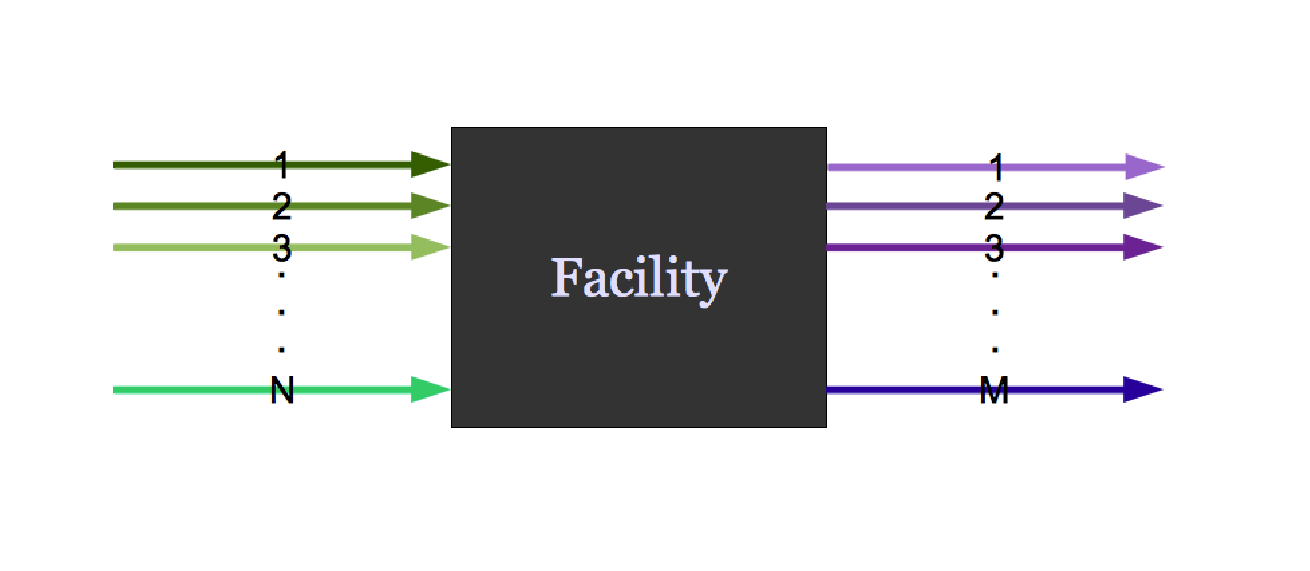
\includegraphics[height=4cm]{./images/facs.eps}
    \caption{Facilities as black boxes. \cite{cyclus2012}.}
    \label{fig:facs}  
  \end{figure}

\end{frame}

\begin{frame}[ctb!]
  \frametitle{Issues with Current Recycled Fuel Matching}
  
  Current implementations of the modeling of recycled fuel fabrication
  \begin{itemize}
    \item lack rigor
    \item don't account for element-isotope issues present at this interface
  \end{itemize}
  
  \vspace{0.2cm}

  VISION models the process by:
  \begin{itemize}
    \item placing separated isotopes in ``bins''
    \item declaring ``control isotopes''
    \item removing the correct control isotopes fraction from the bin
  \end{itemize}
  
\end{frame}

\begin{frame}[ctb!]
  \frametitle{Issues with Current Recycled Fuel Matching}

  COSI's uses the ``Equivalence Model'', adapted from a method introduced in
  1963 by Baker and Ross\cite{baker_comparison_1963}.
  
  \vspace{0.2cm}

  Method and implementation outline:
  \begin{itemize}
    \item used for recycled fuel recipes
    \item assumes ``ideal'' recipe of $^{239}$Pu and $^{238}$U
    \item determines a recipe given ``bins'' of fissile and fertile material
  \end{itemize}
\end{frame}

\begin{frame}[ctb!]
  \frametitle{Issues with Current Recycled Fuel Matching}

  In such a model, the following are defined:
  \begin{itemize}
    \item a quantity of fuel
    \item a target Pu-239 enrichment, $E_0$
    \item a ``bin'' of fertile isotopes
    \item a ``bin'' of fissile isotopes
  \end{itemize}

  And its output is:
  \begin{itemize}
    \item a weight fraction, $E$, to extract from the fissile isotopes
    \item a weight fraction, $1-E$, to extract from the fertile isotopes
  \end{itemize}
\end{frame}

\begin{frame}[ctb!]
  \frametitle{Issues with Current Recycled Fuel Matching}
  
  An isotopic ``worth'' is defined for each isotope, $i$, as:
  \begin{equation}
    w_i = \frac{x_i - x_{^{238}U}}
    {x_{^{239}Pu} - x_{^{238}U}}.
  \end{equation}

  with $x_i$ defined as:
  
  \begin{equation}
    x_i = \nu_{i} \sigma_{f,i} - \sigma_{a,i}
  \end{equation}

  with physical parameters:
  \begin{itemize}
    \item $\nu_{i}$ - average number of neutrons resulting from fission
    \item $\sigma_{f,i}$ - microscopic fission cross section
    \item $\sigma_{a,i}$ - microscopic absorption cross section
  \end{itemize}
\end{frame}

\begin{frame}[ctb!]
  \frametitle{Issues with Current Recycled Fuel Matching} 
  
  With isotopic weight fractions, $\xi_i$, the fissile fraction, $E$, is given
  by:
  \begin{equation}
    E = \frac{E_0 - \sum_{i \in I_{Fe}} \xi_i w_i}
    {\sum_{i \in I_{Fi}} \xi_i w_i - \sum_{i \in I_{Fe}} \xi_i w_i}.
  \end{equation}

  \begin{figure}
    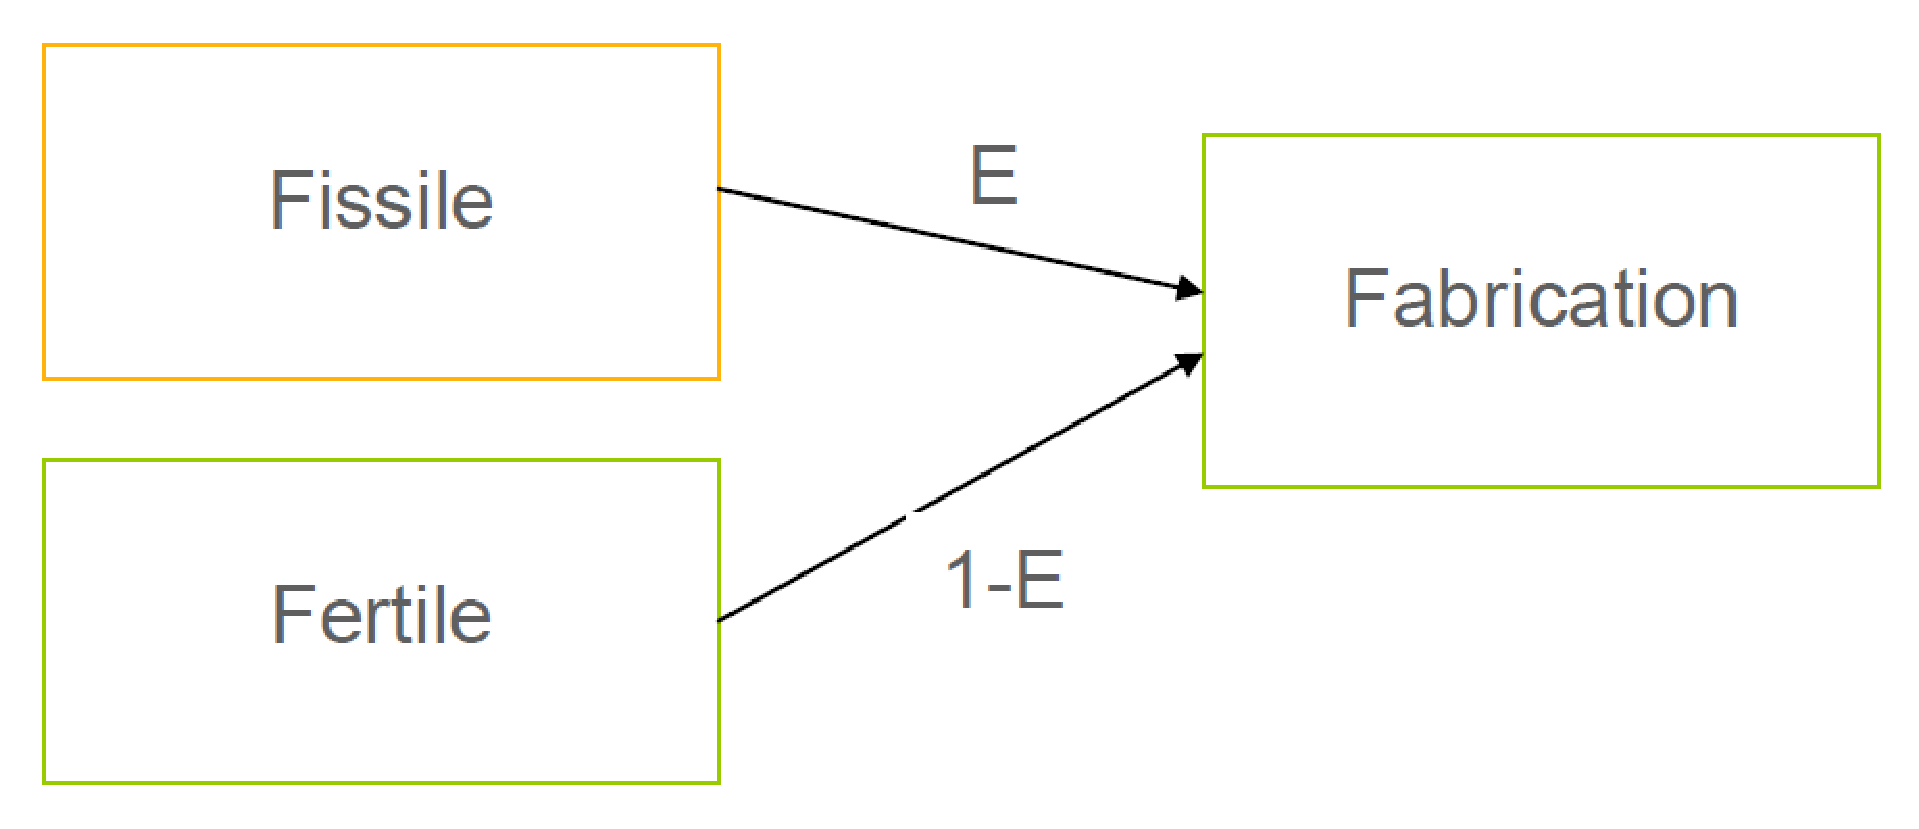
\includegraphics[height=3cm]{./images/equiv.eps}
    \caption{Result of COSI's Equivalence Method. \cite{meyer_new_2009}.}
  \end{figure}
\end{frame}
  
\begin{frame}[ctb!]
  \frametitle{Two Motivating Questions}

  \begin{block}{Dynamic Resource Exchange}
    If facilities are treated as individual black boxes and connections between
    facilities are determined dynamically, how does one match suppliers with
    demanders considering supply constraints and, supply response to
    quality-based demands, and issues of fungibility?
  \end{block}

  \pause

  \begin{block}{Fuel Order Approximation}
    Can one model the interface between separations and recycled fuel
    fabrication more realistically?
  \end{block}

\end{frame}

\section{Proposal}

\begin{frame}[ctb!]
  \frametitle{Resource Exchange Generality}

  To determine a supply-demand resource exchange for \textit{general} facilities
  in the fuel cycle, detailed information about both the supply and demand must
  be known.

  Some examples:
  
  \begin{itemize}
    \item Enrichment facilities - constrained by both quality and quantity of fuel
      requested
    \item Reactors - request specific isotopic profiles for new fuel
    \item Fabrication facilities - must know the isotopic profile of fuel to
      provide
  \end{itemize}
  
\end{frametitle}


\begin{frame}[ctb!]
  \frametitle{Resource Exchange Information Gathering}

  The nuclear fuel cycle has some similarities to the petroleum industry (i.e.,
  the quality of the product must be taken into account), and is a
  \textit{supply chain}.

  \\

  Furthermore, facilities making decisions based on product quality act in an
  agent-like manner.

  \\ 

  Accordingly, I looked toward agent-based supply chain modeling of the
  petroleum industry for inspiration, and have adopted an approach proposed by
  Julka et. al \cite{julka_agent-based_2002} to be used under the proposed
  \Cyclus design constraints.
\end{frame}

\begin{frame}[ctb!]
  \frametitle{Resource Exchange: Request for Bids}
  \begin{figure}
    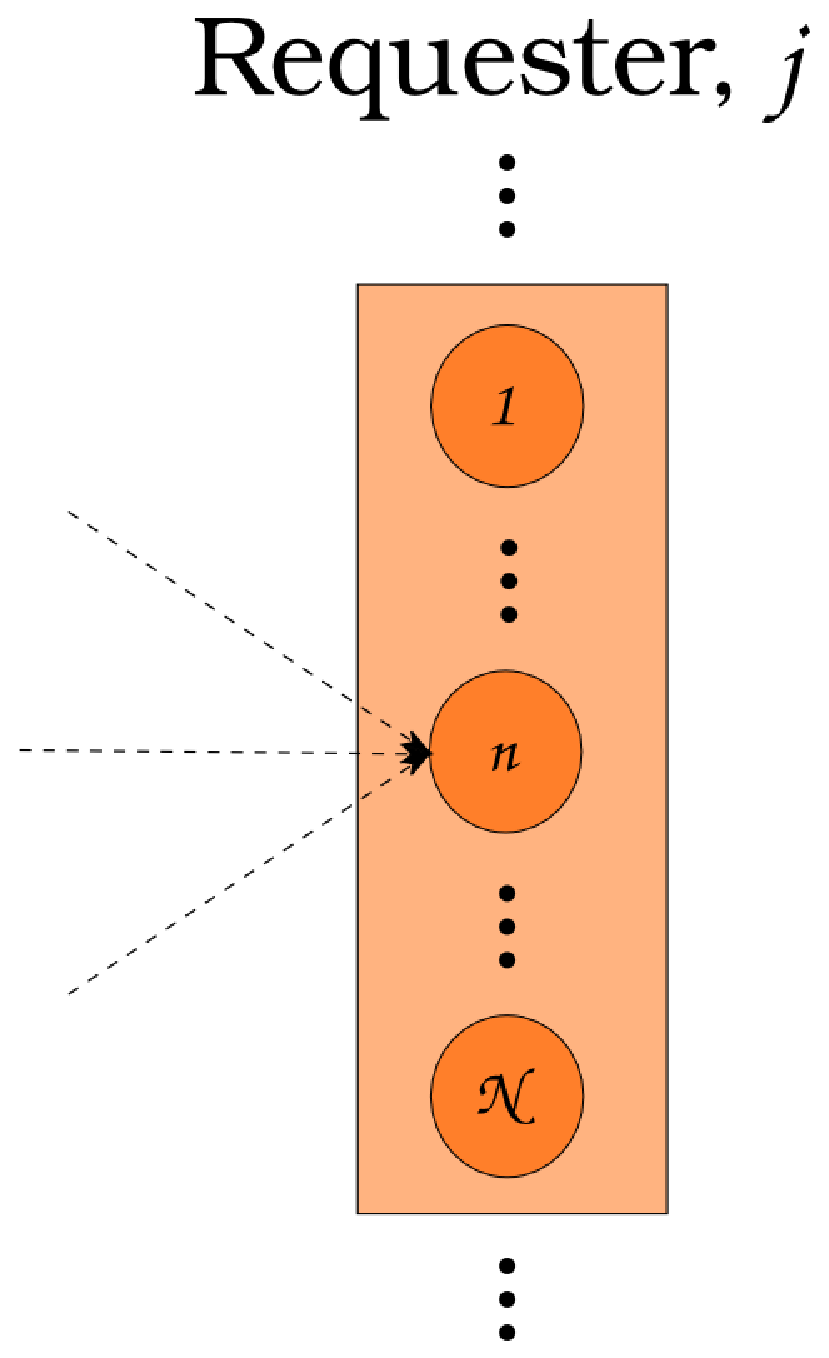
\includegraphics[height=5cm]{./images/requester.eps}
    \caption{Consumers define their demand for commodities during the Request
      for Bids (RFB) phase.}
  \end{figure}
\end{frame}

\begin{frame}[ctb!]
  \frametitle{Resource Exchange: Response to Request for Bids}
  \begin{figure}
    \includegraphics[height=5cm]{./images/suppliers.eps}
    \caption{Suppliers respond to each request during the Response to Request
      for Bids (RRFB) phase.}
  \end{figure}
\end{frame}

\begin{frame}[ctb!]
  \frametitle{Resource Exchange: Preference Adjustment}
  \begin{figure}
    \includegraphics[height=5cm]{./images/suppliers-requesters.eps}
    \caption{Consumers adjust preferences based on Supplier-given information
      during the Preference Adjustment (PA) phase.}
  \end{figure}

  Managers of facilities (institutions, regions) are then allowed to perturb
  preferences.
\end{frame}

\begin{frame}[ctb!]
  \frametitle{Resource Exchange: Full Picture}
  \begin{figure}
    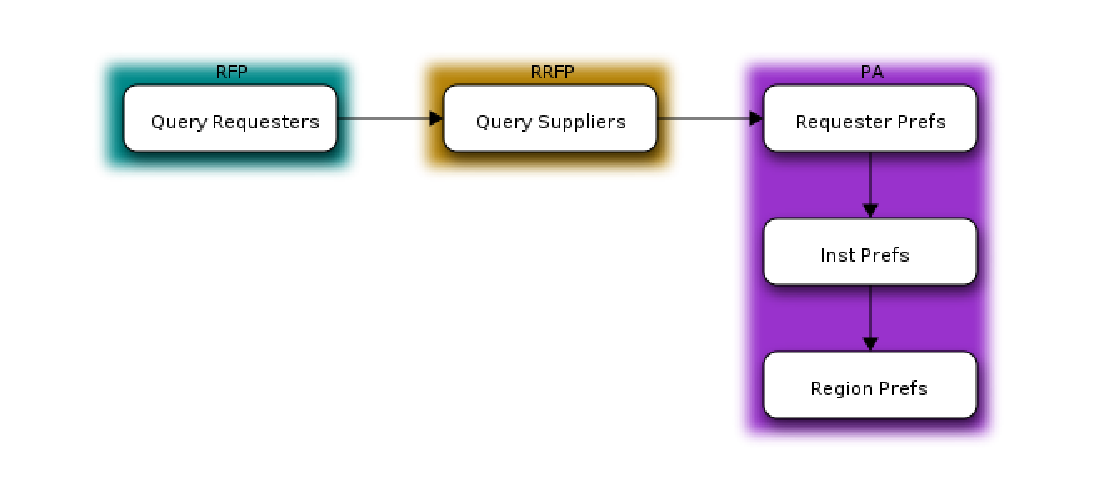
\includegraphics[height=5cm]{./images/exchange.eps}
    \caption{A flow chart of the information gathering phases.}
  \end{figure}
\end{frame}

\begin{frame}[ctb!]
  \frametitle{Resource Exchange Solution Mechanism}
  
  As defined, facilities in \Cyclus are black boxes, but there is a notion of
  supplier and consumer facilities of a variety of commodities.

  \\

  We seek a solution to a flow of (discrete) materials, where for each
  commodity, we have now defined a set of suppliers and consumers of that
  commodity. 

  \\ 
  
  Furthermore, suppliers may be able to provide more than one commodity and
  consumers may be able to consume more than one commodity.

  \\

  Accordingly, a Multicommodity Transportation Problem formulation naturally
  fits the needs of our simulation. Let's call it the Generic Fuel Cycle
  Transportation Problem (GFCTP).
  
\end{frame}


\begin{frame}[ctb!]
  \frametitle{GFCTP - Description}
  
\end{frame}

And an example \cite{hamilton_blue_2012}.
\section{Acknowledgements}
\begin{frame}[ctb!]
  \frametitle{Acknowledgments}
  First and foremost, I would like to thank the members of the
  Computational Nuclear Engineering Research Group at UW 
  \begin{itemize}
    \item Robert Carlsen
    \item Dr. Anthony Scopatz
    \item Dr. Paul Wilson
  \end{itemize}
  
  \vspace{0.2cm}
  
  and prior members:
  \begin{itemize}
    \item Katy Huff
    \item Kyle Oliver
  \end{itemize}

\end{frame}

\begin{frame}[ctb!]
  \frametitle{Acknowledgments}
  And, of course, I would like to thank the DOE Office of Nuclear Energy's 
  Nuclear Engineering University Programs for providing funding. 
  \begin{figure}[htbp!]
    \begin{center}
      
\includegraphics[height=2cm]{neup.ps}
    \end{center}
    \label{fig:neup}
  \end{figure}
\end{frame}


%||||---------------
\begin{frame}[allowframebreaks]
  \frametitle{References}
  \bibliographystyle{plain}
  \bibliography{main}
\end{frame}
%---------------||||




\end{document}
